\documentclass[12pt]{article}

\usepackage{CJKutf8}
% 打中文時請務必加這個Package

\usepackage{epsfig,amsmath,amssymb,latexsym}
\usepackage{graphicx,epsfig,color,epsf,psfrag,hhline,amsmath,amssymb,textcomp}
%\usepackage{hyperref}
\usepackage{enumitem}
\usepackage{subfigure}

\setlength {\topmargin}{-1.0in}
\setlength {\textheight}{10in}
\setlength {\oddsidemargin}{-0.25in}
\setlength {\evensidemargin}{-0.25in}
\setlength {\textwidth}{6.75in}
\setlength {\parskip}{8pt plus 2pt minus 1pt}

\newtheorem{theorem}{Theorem}[section]
\newtheorem{definition}{Definition}[section]
\newtheorem{lemma}{Lemma}[section]

\newcommand{\comb}[2]{\left (\begin{array}{c} #1 \\ #2 \end{array} \right )}

\newcommand{\inlinecomb}[2]{\mbox{\scriptsize $\left (\begin{array}{c} #1 \\ #2 \end{array} \right )$\normalsize}}

\newcommand {\bsolution}{\noindent {\em Solution:} \ }

\newcommand{\esolution}{\hfill $\Diamond$ \\ \vspace{.3cm}}

%************************** Figure**********************************
\newcommand {\bfig}[2] {\begin{figure}[htbp]
                        \centerline {
                         \epsfig{figure={#1},clip=,width={#2}}}}

\newcommand {\efig}[2]{ \caption{#2}
                        \label{fig:#1}
                        \end{figure}
                        \mymarginpar{fig:#1}}
\newcommand {\rfig}[1]{Figure \ref{fig:#1}}

%%%%%%%%%%%%%%%%%%%%%%%%%%%%%%%%%%%%%%%%%%%%%%%%%

\begin{document}
\thispagestyle{empty}
\begin{center}
{\Large \noindent COM 530500 {\bf Network Science Final Project} \\
\large {{\sc Due:} Thursday, January 20, 2022}  \\
}
\emph{No late homework will be accepted}.
\end{center}


\noindent {\begin{CJK}{UTF8}{bsmi}
{\bf 班級:} 資應所
\end{CJK}}

\noindent  {\begin{CJK}{UTF8}{bsmi}
{\bf 姓名:} 鄭程哲
\end{CJK}}

\noindent {\begin{CJK}{UTF8}{bsmi}
{\bf 學號:} 110065512
\end{CJK}}

\bigskip


%---------------------------------------------------------------------------
% Problem 1
%---------------------------------------------------------------------------

\noindent {\bf Problem 1. (40\%)} Consider the {\bf ego-Facebook} \cite{leskovec2012learning} dataset. A node in this dataset represents a user on Facebook, and an edge between two nodes represents the relationship between two users.
\begin{enumerate}[label=(\alph*)]
	\item (10\%) List some statistical information of this dataset, such as the number of nodes, number of edges, average clustering coefficient, diameter, average degree, maximum degree, etc.
	\item (10\%) Visualize the dataset by plotting it.
	\item (10\%) Plot the degree distribution with log-log scale.
	\item (10\%) List the top 10 nodes ranked by the following centrality measures.
	\begin{itemize}
		\item Degree centrality
		\item Katz centrality
		\item Eigenvector centrality
		\item Betweenness centrality
		\item Closeness centrality
	\end{itemize}
\end{enumerate}

\bsolution
%---------------------------------------------------------------------------
\begin{enumerate}[label=(\alph*)]
	\item Statistical information:
	\begin{itemize}
		\item The number of nodes: $2851$
		\item The number of edges: $62318$
		\item Average clustering coefficient: $0.591376$
		\item Diameter: $14$
		\item Average degree: $43.7166$
		\item Maximum degree: $769$
		\item Minimum degree: $1$
		\item Density: $0.01534$
	\end{itemize}
	\item Visualization is as figure 1 show.
	\begin{figure}[h]
		\centering
		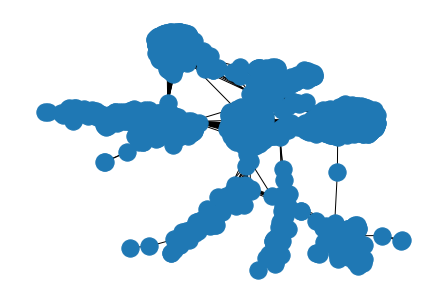
\includegraphics[width=0.6\textwidth]{visualize.png}
		\caption{Visualization}
		\label{visualize}
	\end{figure}
	\item Degree distribution is as figure 2 show.
	\begin{figure}[h]
		\centering
		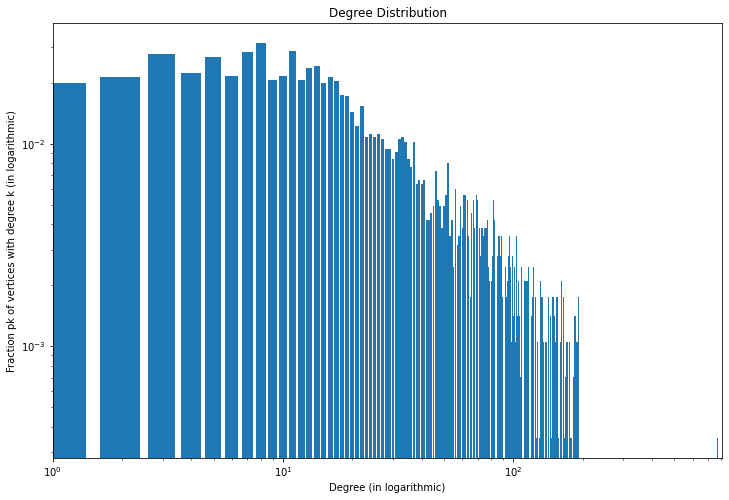
\includegraphics[width=0.8\textwidth]{degree dist.png}
		\caption{Degree distribution}
		\label{degree}
	\end{figure}
	\item 
	\begin{itemize}
		\item Degree centrality: 1165 91 0 1862 1681 1606 288 1341 1575 1298
		\item Katz centrality: 1165 91 1862 1681 0 1606 1341 1575 1298 1493
		\item Eigenvector centrality: 1606 1551 1575 1790 1431 1561 1493 1741 1581 1349
		\item Betweenness centrality: 91 1165 0 1110 611 1056 771 892 1181 351
		\item Closeness centrality: 91 1165 1156 1086 933 1110 1181 1056 147 49
	\end{itemize}
\end{enumerate}
%---------------------------------------------------------------------------
\esolution


%---------------------------------------------------------------------------
% Problem 2
%---------------------------------------------------------------------------

\noindent {\bf Problem 2. (60\%+bonus 10\%)} In this problem, we want to investigate the disease propagation by the independent cascade (IC) model in {\bf ego-Facebook} \cite{leskovec2012learning} dataset. Assume the propagation probability is $\phi$, and the set of seeds nodes $S$ are randomly selected. Collect the set of infected nodes within the distance $D$ of the seed nodes, and calculate the prevalence rate $r_1$ (which is defined by the ratio of the number of infected nodes to the total number of nodes). Set $\phi=0.1, \vert S \vert=5$, and $D$ the diameter of the graph.

\begin{enumerate}[label=(\alph*)]
	\item (40\%) Simulate the disease propagation by IC model after removing the top $0\%$, $10\%$, $20\%$, $\ldots$, $50\%$ of nodes from the following centrality measures respectively, and calculate the corresponding prevalence rate $r_1$. Please plot the curves of $r_1$ vs. the percentage of nodes removed. ({\it Note: Please run the simulation 100 times and average the results.})
	\begin{itemize}
		\item Degree centrality
		\item Katz centrality
		\item Eigenvector centrality
		\item Betweenness centrality
		\item Closeness centrality
	\end{itemize}
	\item (bonus 10\%) Could you find a centrality measure that achieves a better performance?
	\item (20\%) Write a report to compare and discuss the results of different centrality measures.  
\end{enumerate}

\bsolution
%---------------------------------------------------------------------------
\begin{enumerate}[label=(\alph*)]
	\item The experiment results are shown as the following table and figure 3. The bold text in the table means the lowest $r1$ comparing to the other measures. In figure 3(b), I additionally plot the box information corresponding to different measures. \\[1em]
		\begin{tabular}{|c|l|l|l|l|l|l|}
			\hline
			Measure     & 0\% & 10\% & 20\% & 30\% & 40\% & 50\% \\ \hline
			Degree      & 0.689032 & 0.374749 & 0.120698 & \textbf{0.010463} & \textbf{0.002925} & \textbf{0.002066} \\ \hline
			Katz        & \textbf{0.687464} & 0.435170 & 0.157306 & 0.026429 & 0.004037 & 0.002413 \\ \hline
			Eigenvector & 0.689747 & 0.548369 & 0.339309 & 0.186615 & 0.072929 & 0.027938 \\ \hline
			Betweenness & 0.695184 & \textbf{0.226962} & \textbf{0.094949} & 0.039646 & 0.011122 & 0.002434 \\ \hline
			Closeness   & 0.693094 & 0.339548 & 0.200284 & 0.110716 & 0.047341 & 0.022210 \\ \hline
		\end{tabular} \\	
		\begin{figure}[htbp]
			\centering
			\subfigure[Line chart]{
				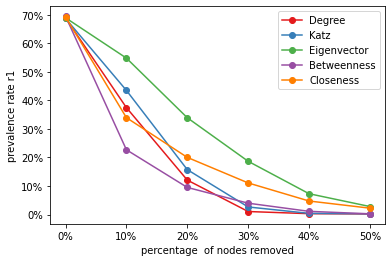
\includegraphics[width=0.6\textwidth]{r1.png}
				\label{r1}
			}
			\quad
			\subfigure[Line chart with box]{
				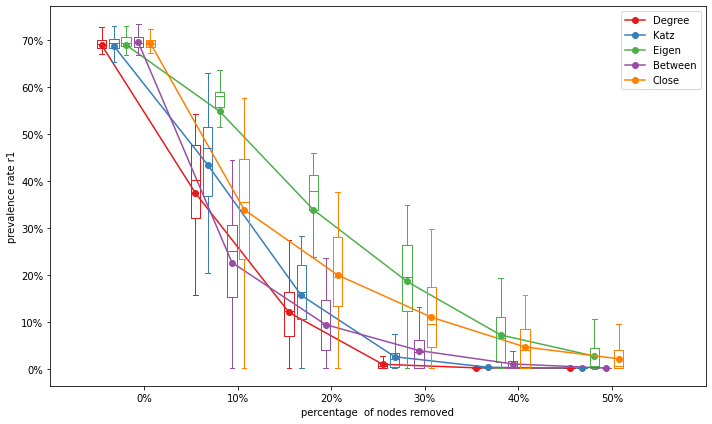
\includegraphics[width=0.8\textwidth]{r1_box.png}
				\label{r1_box}
			}
			\caption{$r1$ curve corresponding to different measures and percentage}
		\end{figure}
	\\
	\item I tried other different centrality measures including PageRank, VoteRank, and Harmonic centrality. The experiment results are shown as figure 4. As we can see from the table below, PageRank breaks two best records, which are $20\%$ and $50\%$, respectively. I think PageRank is a quite good centrality measure. Further discussion would be written in the part (c). In contrast, VoteRank and harmonic centrality measures didn't have a better performance. \\ [1em]
		\begin{tabular}{|c|l|l|l|l|l|l|}
			\hline
			Measure       & 0\% & 10\% & 20\% & 30\% & 40\% & 50\% \\ \hline
			Best from (a) & \textbf{0.687464} & \textbf{0.226962} & 0.094949 & \textbf{0.010463} & \textbf{0.002925} & 0.002066 \\ \hline
			PageRank      & 0.689937 & 0.276692 & \textbf{0.084177} & 0.015167 & 0.004504 & \textbf{0.001884} \\ \hline
			VoteRank      & 0.688888 & 0.280277 & 0.086461 & 0.040621 & 0.008362 & 0.009404 \\ \hline
			Harmonic      & 0.694942 & 0.333560 & 0.176552 & 0.092083 & 0.033385 & 0.018622
			 \\ \hline
		\end{tabular} \\
		\begin{figure}[htbp]
			\centering
			\subfigure[Line chart]{
				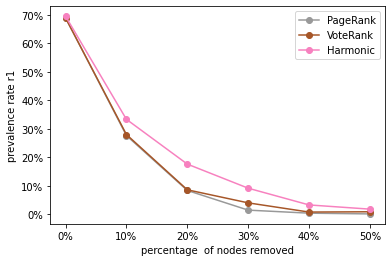
\includegraphics[width=0.6\textwidth]{r1_other.png}
				\label{r1_other}
			}
			\quad
			\subfigure[Line chart with box]{
				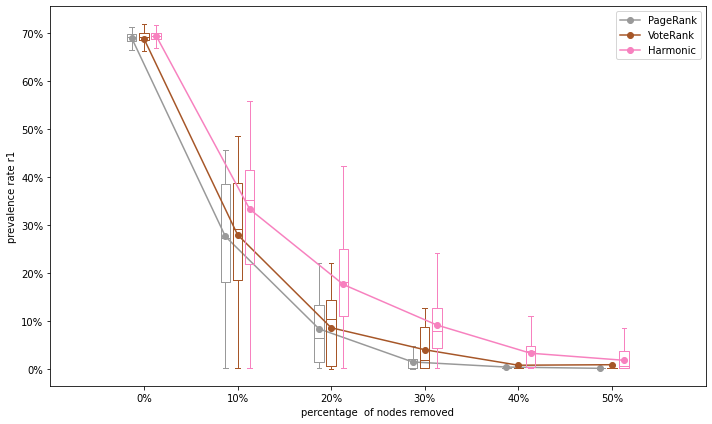
\includegraphics[width=0.8\textwidth]{r1_other_box.png}
				\label{r1_other_box}
			}
			\caption{$r1$ curve corresponding to other measures}
		\end{figure}
	\\ \\ \\
	\item Removing $0\%$ vertices has no difference for different measures, so we can ignore this column. When the percentage of node removal is low (10\%, 20\%), $r1$ drops a lot with betweenness, PageRank, and VoteRank measures. That is, applying this concept into real world, we can use these 3 measures to reduce $r1$ efficiently when the shortage of vaccine occurs.\\ \\
	For another thing, degree centrality achieves 2 best $r1$, betweenness centrality achieves 1 best $r1$, and PageRank achieves 2 best $r1$ in total. In figure 5, I plot more details about these 3 good measures. The dot in the plot means the average value of $r1$, while the shaded area represents $\pm 1$ standard deviation of mean. As we can see from the figure, the higher percentage of nodes removal, the performance converge more tightly. In other words, the variance of performance is higher if the shaded area is bigger. The performance with high variance would be not accurate. Although both degree centrality and PageRank has 2 best $r1$ records, PageRank achieves the best performance in $50\%$ nodes removal. \\ \\
	Combining above two points, I, therefore, think PageRank is the best centarlity measures among all in this task.
		\begin{figure}[htbp]
			\centering
			\subfigure[Degree centrality]{
				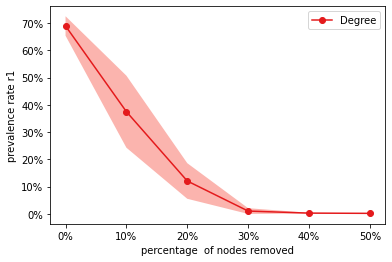
\includegraphics[width=0.4\textwidth]{r1_degree.png}
				\label{r1_degree}
			}
			\quad
			\subfigure[Betweenness centrality]{
				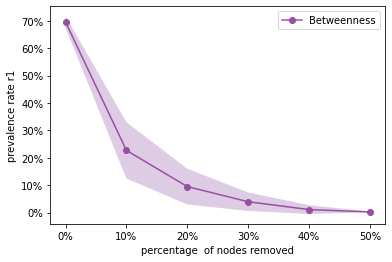
\includegraphics[width=0.4\textwidth]{r1_betweenness.png}
				\label{r1_betweenness}
			}
			\quad
			\subfigure[PageRank]{
				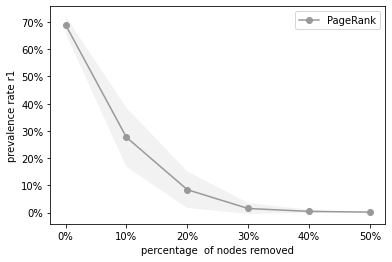
\includegraphics[width=0.4\textwidth]{r1_pagerank.png}
				\label{r1_pagerank}
			}
			\caption{$r1$ curve corresponding to a specific measure}
		\end{figure}
\end{enumerate}
%---------------------------------------------------------------------------
\esolution

%---------------------------------------------------------------------------
% The end of problems.
%---------------------------------------------------------------------------

%---------------------------------------------------------------------------
\iffalse
\noindent {\bf Given}: adjacency matrix $A$, transition probability $\phi$, a set of seed nodes $S$, and distance $D$.

\noindent {\bf Step 1}: Obtain $A^\prime$ by removing edges of $A$, where each edge is removed with probability $1-\phi$.

\noindent {\bf Step *}: {\bf Obtain $\tilde{A}$ by removing some specific nodes and all their edges from $A^\prime$.}

\noindent {\bf Step 2}: Define the $n \times 1$ seed vector $x$ by $x_i=1$ for $i \in S$ and $x_i=0$ for $i \notin S$.

\noindent {\bf Step 3}: Calculate $y=(\tilde{A}+I)^Dx$ with the AND and the OR operations.

\noindent {\bf Step 4}: Obtain the number of infected nodes by counting the number of 1's in vector $y$.

\noindent {\bf Step 5}: Repeat {\bf Step 1} to {\bf Step 5} for $100$ times, and average the results.

\noindent {\bf Step 6}: Calculate the prevalence rate $r_1$.
\fi
%---------------------------------------------------------------------------

%---------------------------------------------------------------------------
% References
%---------------------------------------------------------------------------
\begin{thebibliography}{9}
\bibitem{leskovec2012learning}
J.~Leskovec and J.~J. Mcauley, ``Learning to discover social circles in ego networks,'' in \emph{Advances in neural information processing systems},
2012, pp. 539--547.

\end{thebibliography}

\end{document}
